\documentclass[12pt]{article}
%\documentclass[12pt,a4paper]{article}
%Size -- the best choice for university course
%slides seems landscape A5, 12pt letters.  Margins
%are made narrow, as much text on each page as possible.

%Could define size explicitly, but finally A5 was selected:

\usepackage[%paperwidth=600pt,paperheight=450pt,
a5paper,left=15pt,right=15pt,top=3pt,bottom=3pt,%
  %outer=25mm,
  %inner=35mm,
  %vmargin=2mm,
  includehead,includefoot,headheight=15.4pt,headsep=5pt,%
  footskip=22pt,landscape]{ geometry }


\usepackage{tocloft}
%\usepackage{tocloft}% http://ctan.org/pkg/tocloft
\setlength{\cftsecnumwidth}{1.9em}
\setlength{\cftsubsecnumwidth}{2.95em}
\setlength{\cftsubsubsecnumwidth}{3.7em}
% Set length of number width in ToC
% so that the number has enough space and
% does not run into the subsection title.

\usepackage[unicode,colorlinks=true,breaklinks]{hyperref}
%\usepackage[dvips]{hyperref}
%should display links, but it does not work with \H accent
%and formulas in section titles

\hypersetup{colorlinks,%
  linkcolor=blue,urlcolor=magenta,citecolor=green}
%Breaks long url`s in text, while keeping it one link:
\usepackage{breakurl}

\newcommand{\nc}{\newcommand} % a newcommand rövidítése
\newcommand{\rc}{\renewcommand} % a renewcommand rövidítése

\newcommand{\bb}[1]{\mathbf{#1}}
\newcommand{\dd}{\mathrm{d}}

%Creates header and footer w time, section titles, etc. 
%Here the stripes are made narrow. 
\usepackage{fancyhdr}
\usepackage[yyyymmdd,hhmmss]{datetime}

\pagestyle{fancy}
\rc{\headrulewidth}{0.3pt}
\rc{\footrulewidth}{0.3pt}
\lfoot{\today\, \currenttime}
\cfoot{}
\rfoot{\thepage}

\sloppy %To prefer larger spaces between 

%words rather than overflow a line. 
\frenchspacing %No wide space after period, this is the
%French and also the Hungarian rule. 

\usepackage{bookmark}
\usepackage[medium,compact,toctitles]{titlesec}
\usepackage[active]{srcltx}
\usepackage{braket}
%\usepackage{savetrees} 
% others: 

\usepackage{t1enc}
\usepackage{amsmath, amssymb, amsfonts, amsbsy, amsthm}
\usepackage{mathtools}
\usepackage{soul} % For \st command
\let\equation\gather
\let\endequation\endgather

%\usepackage[magyar]{babel}
\usepackage[utf8]{inputenc} 
%\usepackage[pdftex]{graphicx}

\usepackage{graphicx}
%\graphicspath{{./}{kepek/}{./files/}}

\usepackage{epstopdf}
\epstopdfsetup{update}
% only regenerate pdf files when eps file is newer



\usepackage[width=.75\textwidth]{caption}
\usepackage{lmodern}%Avoid rastering for letters.  
 
% Alább definiáljuk a magyar névelőhöz illeszkedő egyenlet hivatkozást.
% A magyar csomag része \az{..} az argumentumbeli számnévhez 
% illeszkedő névelő, \Az ugyanez % nagybetűvel, ezeket használjuk 
% alább.  
\nc{\Aeqref}[1]{\Az{\eqref{#1}}}
\nc{\aeqref}[1]{\az{\eqref{#1}}}

\usepackage{bbold}
\usepackage{ulem}
\usepackage[caption=false]{subfig} 
%\usepackage{epsfig}
%\usepackage[dvips]{color}
\usepackage{accents}
\usepackage{bbold}
\usepackage{textcomp}
\usepackage{nicefrac}%\nicefrac{}{} makes frac with slash for text
\usepackage[section]{placeins} %have \FloatBarrier,
%issued automatically at section titles 

\usepackage{wrapfig} %for wrapping text around floats 
\usepackage{indentfirst}
%for indenting the first para after section title, customary in 
%Hungarian but not so in English.  
\usepackage[integrals]{wasysym} %symbols for planets 
\usepackage{upgreek}
\usepackage{bm}\usepackage{bbm}
%I experimented with those:
%\usepackage[utopia]{mathdesign}
%\usepackage[OMLmathrm,OMLmathbf]{isomath}
%\usepackage{movie15}
%\usepackage[thinlines]{easytable} % DOES NOT WORK!
%comfortable table creation
%\begin{TAB}(r,1cm,2cm)[5pt]{|l|}{|c|c|}
%(rows,min,max)[tabcolsep]{columns}{rows}
%\end{TAB}


\rc*\familydefault{\sfdefault}
%entire doc in sanserif for better reading from projection

%redefine paragraph to enumerate them
\setcounter{secnumdepth}{6}
\rc\theparagraph{{\it\bf\alph{paragraph}}}
\rc\thesubparagraph{{\it\bf\roman{subparagraph}}}

\makeatletter
\rc\paragraph{\@startsection{paragraph}{4}{\z@}
{-3.25ex\@plus -1ex \@minus -.2ex}%
{5pt \@plus .2ex}%
{\normalfont\normalsize\bfseries\itshape}}
\rc\subparagraph{\@startsecton{paragraph}{5}{\z@}%
{-3.25ex\@plus -1ex \@minus -.2ex}%
{5pt \@plus .2ex}%
{\normalfont\normalsize\itshape}}

% \rc*\itemize{%
%   \ifnum \@itemdepth >\thr@@\@toodeep\else
%     \advance\@itemdepth\@ne
%     \edef\@itemitem{labelitem\romannumeral\the\@itemdepth}%
%     \expandafter
%     \list
%       \csname\@itemitem\endcsname
%       {\def\makelabel##1{\hss\llap{##1}}%
%        \setlength{\itemsep}{2pt}%
%        \setlength{\parsep}{2pt}%
%        \setlength{\parindent}{7pt}}%
%   \fi}

\makeatother

%\rc{\labelitemi}{$\to$}
%\rc{\labelitemii}{$\star$}



%Az "innen következik" jel formulában 
% \nc{\ra}{ \ \ \leadsto \ \ } %Ezen kicsi a nyíl.

% \nc{\el}{\mathcal{E}}

%számozott műfajok 
%\newtheorem{hf}{\text{\it Házi feladat}}[section]
%\nc{\HF}[1]{{\hf \tc{MB}{#1}}}
% \newtheoremstyle{mystyle}
% {headspec} \thmnumber{ #1} \thmname{#2} \thmnote{#3}
% \newtheorem{gf}{\text{\it{\cya{Gyakorló feladat}}}}[section]
% \nc{\GF}[1]{{\gf #1}}
% \nc{\GFL}[2]{{\begin{gf}\label{gf:#2} #1\end{gf}}}
% \nc{\GFN}[1]{{\vspace{-0.5\baselineskip}\gf #1}}
% \newtheorem{pl}{\text{\it{{Példa}}}}[subsection]

% \usepackage{xpatch}
% \makeatletter
% \xpatchcmd{\@thm}{\thm@headpunct{.}}{\thm@headpunct{}}{}{}
% \makeatother

% \nc{\PL}[1]{{\pl \gre{#1}}}
% \nc{\PLL}[2]{{\begin{pl}\label{pl:#2} \gre{#1}\end{pl}}}
% \nc{\dl}[2]{\hfill\yel{$2016.#1  \ \blacktriangleleft \ %
% \mid \ \blacktriangleright \ 2016.#2$}}%az előadások dátumai
% \nc{\dln}[2]{\hfill\yel{$2017.#1  \ \blacktriangleleft \ %
% \mid \ \blacktriangleright \ 2017.#2$}}%az előadások dátumai



%praktikus: vb soremelés, vbn állítható, nn egyenlet végére
\nc{\vb}{\vspace{\baselineskip}}
\nc{\vbn}[1]{\vspace{#1\baselineskip}}
\nc{\nn}{\nonumber}

%\numberwithin{equation}{subsection}
\numberwithin{equation}{section}
\usepackage{cleveref}

\setlength{\parskip}{0.3\baselineskip}
%\setlength{\itemsep}{-0.3\baselineskip} --- does not work
%\setlength{\itemsep}{2pt plus2pt minus2pt} --- does not work
\AtBeginDocument{\addtocontents{toc}{\protect\setlength{\parskip}{0pt}}}
%do not loosen toc by possibly large parskip
\linespread{0.93} %compactify

%compactify
\setcounter{topnumber}{2}
\setcounter{bottomnumber}{2}
\setcounter{totalnumber}{4}
\rc{\topfraction}{0.85}
\rc{\bottomfraction}{0.85}
\rc{\textfraction}{0.15}
\rc{\floatpagefraction}{0.7}
\rc{\theHequation}{\theHsection\arabic{equation}}
%needed for hyperref


% \usepackage{movie15} % to include movies
% \usepackage{hyperref} % prerequisite for movie15 -- these do not seem 
% to work includeonly{em0.1,em1.8} % selects from include list below, 
% but uses the other aux files and keeps eq. and sec. numberings mostly 
% correct; omitting includeonly results in including all items -- then 
% \include is equivalent to \clearpage\input{file}\clearpage.
% each included file gets its own .aux file by include
% \include{em0.1} etc.

% Below we use \input, very simple.
\begin{document}

\begin{center}

\thispagestyle{empty}

\rule{10 cm}{2pt}

\vspace{1.5cm}
{ \Large Kwant project}

\vspace{1.0cm}
Nagy Dániel

\vspace{0.5cm}
Week 8: april 7. - april 14. \\
Topological Anderson Insulator 2.

\vspace{0.5cm}
\today

\vspace{0.25cm}
\rule{10 cm}{2pt}

\end{center}
\newpage

%\setcounter{page}{2}
%\tableofcontents
\newpage
\phantomsection

\section{Schedule for the semester}
\begin{table}[ht]
  \centering
  \caption{Original schedule}
  \begin{tabular}{|c|c|}
  \hline
  Week & Scheduled Task \\ [0.5ex]  \hline % inserts table %heading
  feb. 18. - feb. 24. & Installing Kwant \& Running an example \\ \hline
  feb. 25. - mar. 3. & Reading the documentation \& Running more examples \\ \hline
  mar. 4 - mar. 10 & Reading theory of 2DEG \& Writing a 2DEG calculation \\ \hline 
  mar. 11. - mar. 17. & 2DEG constriction in a magnetic field \\ \hline
  mar. 18. -  mar. 24. & Graphene focusing \\ \hline
  mar. 25. -  mar. 31. & Mid term report \\ \hline
  apr. 1. -  apr. 7. & Topological Anderson Insulator/ Majorana fermion 1. \\ \hline
  apr. 8. -  apr. 14. & Topological Anderson Insulator/ Majorana fermion 2. \\ \hline
  easter holiday & - \\ \hline
  apr. 22. - apr. 28. & Topological Anderson Insulator/ Majorana fermion 3. \\ \hline 
  apr. 29. - may 5. & Topological Anderson Insulator/ Majorana fermion 4. \\ \hline 
  Eötvös/Pázmány days & - \\ \hline
  may 13. - may 19. & Final report \\ \hline

  \end{tabular}
\end{table}

\newpage
\begin{table}[ht]
  \centering
  \caption{Status}
  \begin{tabular}{|c|c|}
  \hline
  Week & Scheduled Task \\ [0.5ex]  \hline % inserts table %heading
  feb. 18. - feb. 24. & Installing Kwant \& Running an example  \checkmark \\ \hline
  feb. 25. - mar. 3. & Reading the documentation \& Running more examples \checkmark \\ \hline
  mar. 4 - mar. 10 & Struggling with graphene minimal conductivity - no result \\ \hline 
  mar. 11. - mar. 17. & 2DEG basics \& Eigenstates and LDOS calculation \checkmark \\ \hline
  mar. 18. -  mar. 24. & 2DEG in magnetic field \checkmark \\ \hline
  mar. 25. -  mar. 31. & Mid term report \\ \hline
  apr. 1. -  apr. 7. & Topological Anderson Insulator/ Majorana fermion 1. \\ \hline
  apr. 8. -  apr. 14. & Topological Anderson Insulator/ Majorana fermion 2. \\ \hline
  easter holiday & - \\ \hline
  apr. 22. - apr. 28. & Topological Anderson Insulator/ Majorana fermion 3. \\ \hline 
  apr. 29. - may 5. & Topological Anderson Insulator/ Majorana fermion 4. \\ \hline 
  Eötvös/Pázmány days & - \\ \hline
  may 13. - may 19. & Final report \\ \hline

  \end{tabular}
\end{table}

\newpage
\section{Progress so far}
\begin{itemize}
  \item Installing kwant 1.4.0 
  \item Getting familiar with kwant: Sites, hoppings, builders
  \item Creating simple and more complex tight-binding systems
  \item Calculating transmission coefficients between two leads
  \item Calculating eigenfunctions, local densities of states
  \item Applying homogeneous magnetic field to a quantum point contact
  \item Experimenting with graphene: Minimal conductivity near Dirac-point
\end{itemize}

\newpage
\section{Progress in this week}
\begin{itemize}
  \item Improved on my report
  \item Reading an article: Topological Anderson Insulator \url{https://arxiv.org/abs/0811.3045}
  \item Reading about majorana fermions: 
  \\ Introduction to topological superconductivity and Majorana fermions: \url{http://arxiv.org/abs/1206.1736v2}, 
  \\ Majorana chain in a quantum dot-superconductor linear array: \url{https://arxiv.org/abs/1111.6600},
  \\ Search for Majorana fermions in superconductors: \url{https://arxiv.org/abs/1112.1950}
  \item Trying to understand and reproduce the results described in the article about TAI (\url{https://arxiv.org/abs/0811.3045})
\end{itemize}

\section{Topological insulator theory}
\begin{minipage}[c]{0.45\textwidth}
  \begin{itemize}
    \item Behave as an insulator in the interior, but have conducting edge states
    \item Quantum Hall effect creates protected edge states using a strong magnetic field
    \item Introducing magnetic field breaks time-reversal symmetry
  \end{itemize}
\end{minipage}
\hfill
\begin{minipage}[c]{0.45\textwidth}
  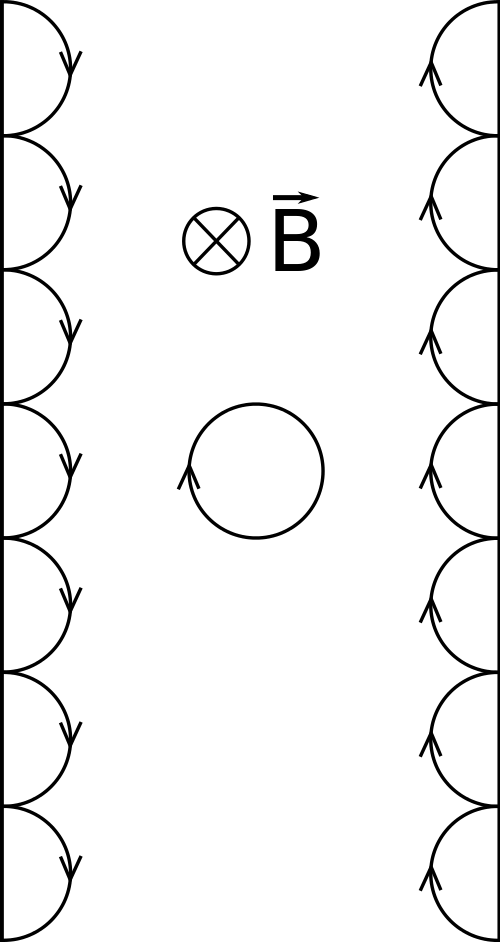
\includegraphics[height=0.75\textheight]{./media/edge_channels_sketch.png}
\end{minipage}


\begin{minipage}[c]{0.45\textwidth}
  \begin{itemize}
    \item Another way to create protected edge states is to start from a system with Dirac cones, and open gaps in those
    \item Graphene is a two-dimensional system which has Dirac cones
    \item This makes graphene suitable to be used as a topological insulator
  \end{itemize}
\end{minipage}
\hfill
\begin{minipage}[c]{0.45\textwidth}
  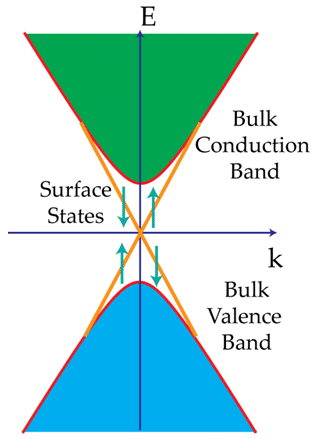
\includegraphics[height=0.75\textheight]{./media/TI-band-structure.png}
\end{minipage}

\newpage
\begin{minipage}[c]{0.4\textwidth}
  \begin{equation*}
    H_0(\mathbf{k})= \begin{pmatrix} 0 & h(\mathbf{k}) \\ h^\dagger(\mathbf{k}) & 0 \end{pmatrix}
  \end{equation*}
  where $\mathbf{k}=(k_x, k_y)$, and
  \begin{equation*}
    h(\mathbf{k}) = t_1\sum_i\exp\left(i\mathbf{k}\cdot\mathbf{a}_i\right)
  \end{equation*}
  Rewritten: 
  \begin{equation*}
    H_0(\mathbf{k}) = t_1\sum_i\left[\sigma_x\cos(\mathbf{k}\cdot\mathbf{a}_i)-\sigma_y \sin(\mathbf{k}\cdot\mathbf{a}_i)\right]
  \end{equation*}
  \begin{equation*}
    E(\mathbf{k}) = \pm \left|h(\mathbf{k})\right| \,\leftarrow \textrm{Dirac cone}
  \end{equation*}
\end{minipage}
\hfill
\begin{minipage}[c]{0.6\textwidth}
  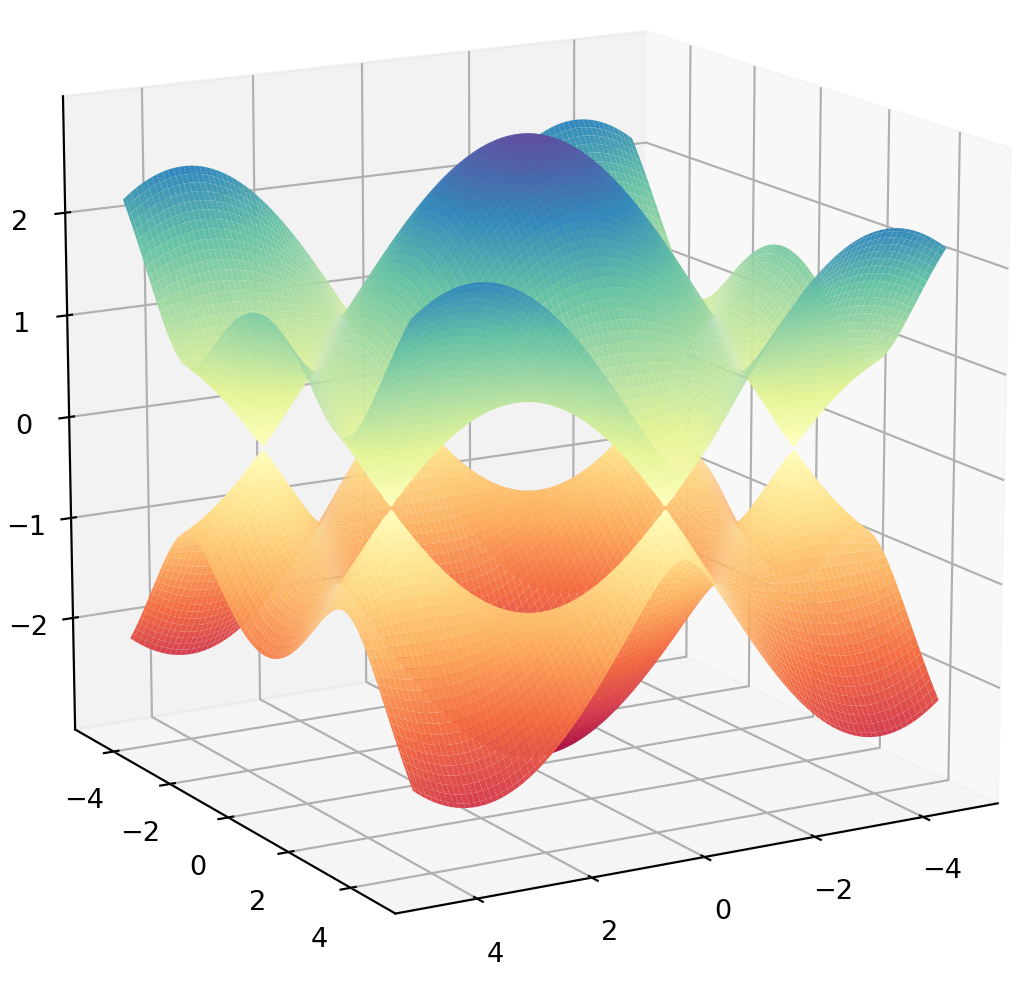
\includegraphics[width=\textwidth]{./media/bulk_graphene_bands_3d_cropped.png}
\end{minipage}




% \newpage
% \begin{figure}[h!]
%   \begin{center}
%   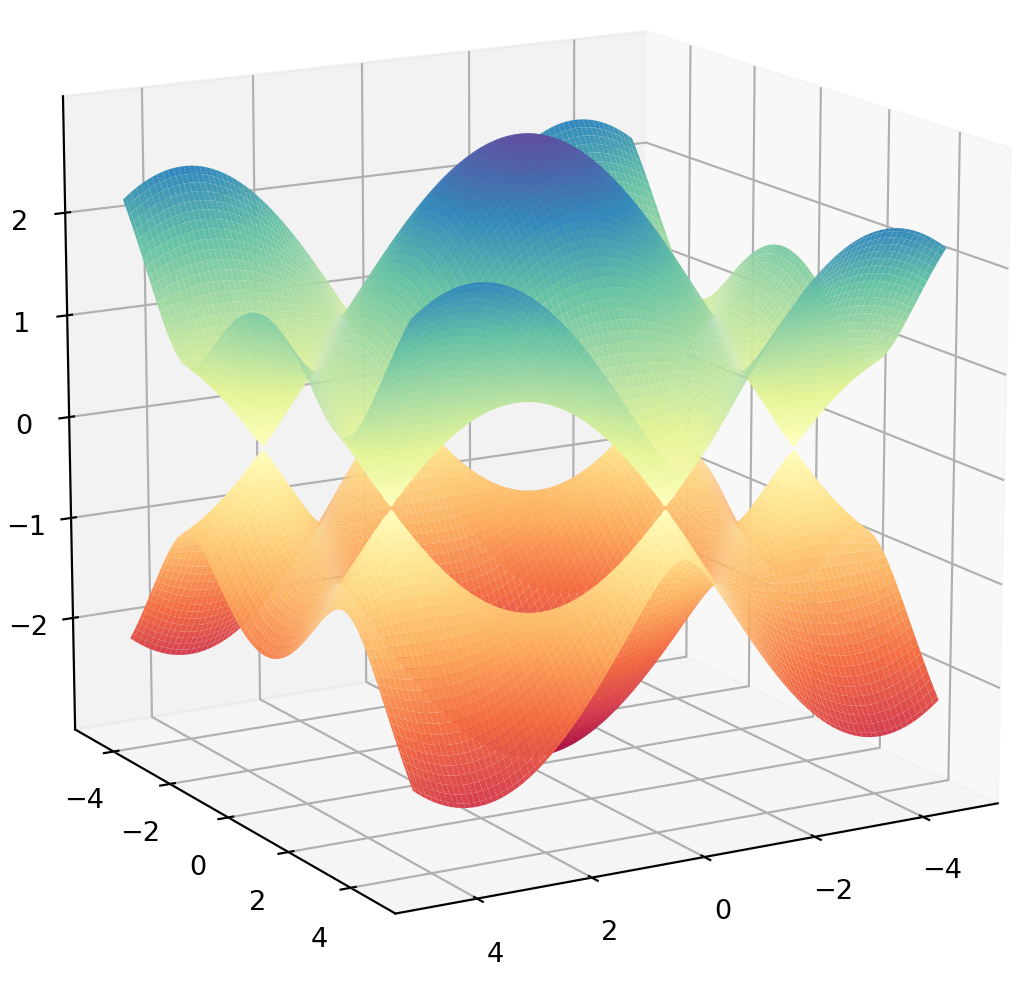
\includegraphics[height=0.85\textheight]{./media/bulk_graphene_bands_3d_cropped.png}
%   \caption{Bandstructre of  bulk graphene plotted with kwant}
%   \label{fig:bsbulk3d}
%   \end{center}
% \end{figure}

\newpage
\begin{minipage}[c]{0.4\textwidth}
  Adding second neighbor hoppings according to Haldane (paper: \url{https://journals.aps.org/prl/abstract/10.1103/PhysRevLett.61.2015})
  \begin{equation*}
    H =  - t\sum\limits_{\left\langle {i,j} \right\rangle \alpha } {c_{i\alpha }^\dagger {c_{j\alpha }}}  + i{\lambda _{SO}}\sum\limits_{\left\langle {\left\langle {i,j} \right\rangle } \right\rangle \alpha \beta } {{\nu _{ij}}c_{i\alpha }^\dagger \sigma _{\alpha \beta }^z{c_{j\beta }}} 
  \end{equation*}
\end{minipage}
\hfill
\begin{minipage}[c]{0.6\textwidth}
  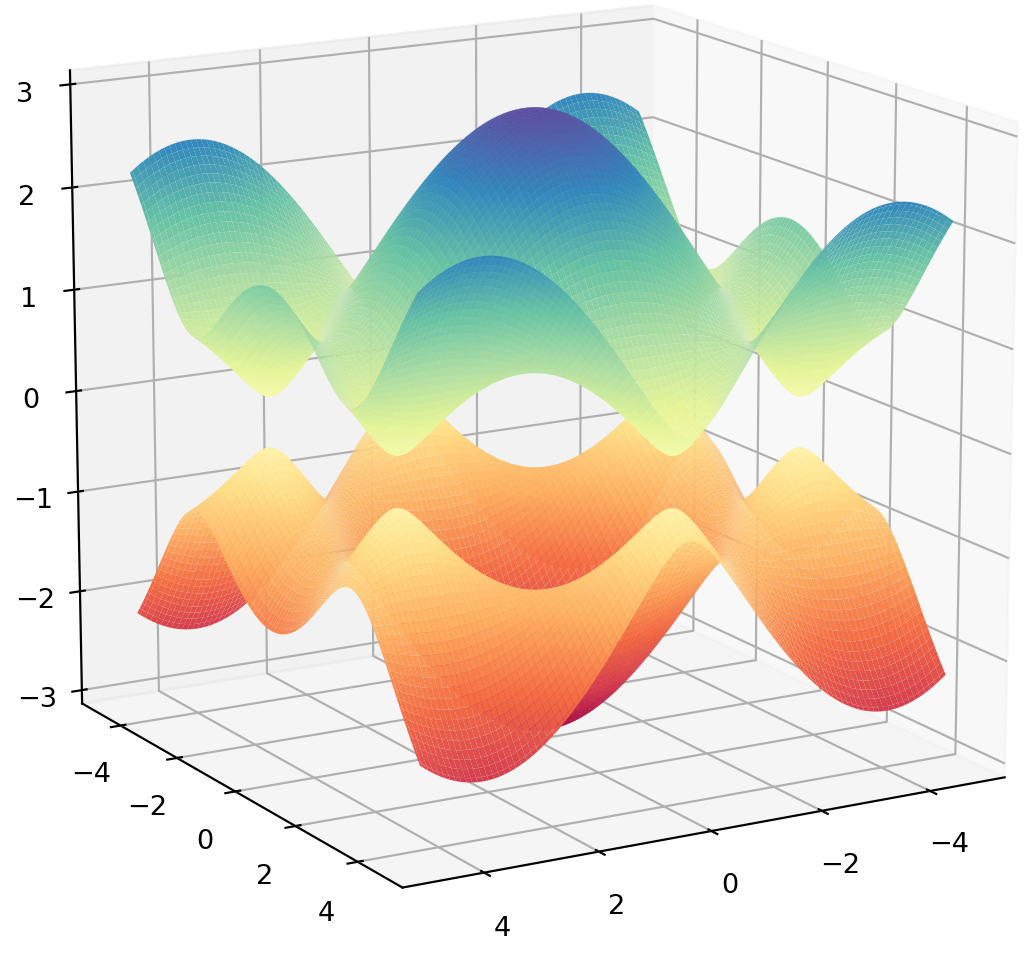
\includegraphics[width=\textwidth]{./media/haldane_bandstruct_t2=0_m=0dot25-cropped.png}
\end{minipage}

% \newpage
% \begin{figure}[h!]
%   \begin{center}
%   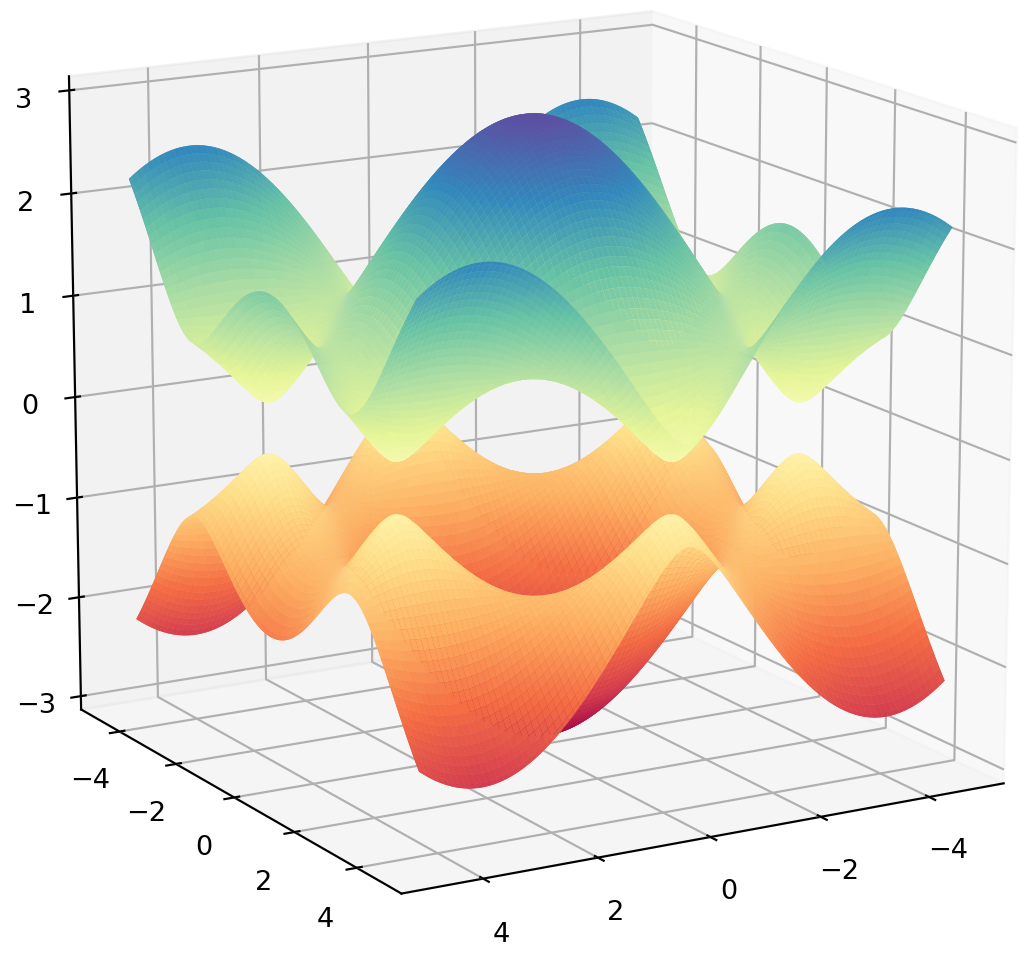
\includegraphics[height=0.85\textheight]{./media/kane-mele-t_2=0_m=0dot25-cropped.png}
%   \caption{Bulk Graphene band structure calculated according to the Kane-Mele model}
%   \label{fig:kanemele3d}
%   \end{center}
% \end{figure}

\newpage
\section{Topological Anderson Insulator}
What are topological Andreson insulators?
\url{https://arxiv.org/abs/0811.3045}


\begin{minipage}[c]{0.45\textwidth}
  \begin{itemize}
    \item The physics of a topological insulator is unaffected by weak
    disorder, but is destroyed by large disorder
    \item BUT: Disorder can create a topological insulator for parameters where the system was metallic in 
    the absence of disorder
    \item These states are called topological Anderson insulators
    \item Disorder can be modeled as random on-site energy with a uniform distribution within $[-W/2, W/2]$
    \item the article discusses disordered strips of HgTe/CdTe quantum wells.
    \item The expected result can be seen on the image
  \end{itemize}
\end{minipage}
\hfill
\begin{minipage}[c]{0.5\textwidth}
  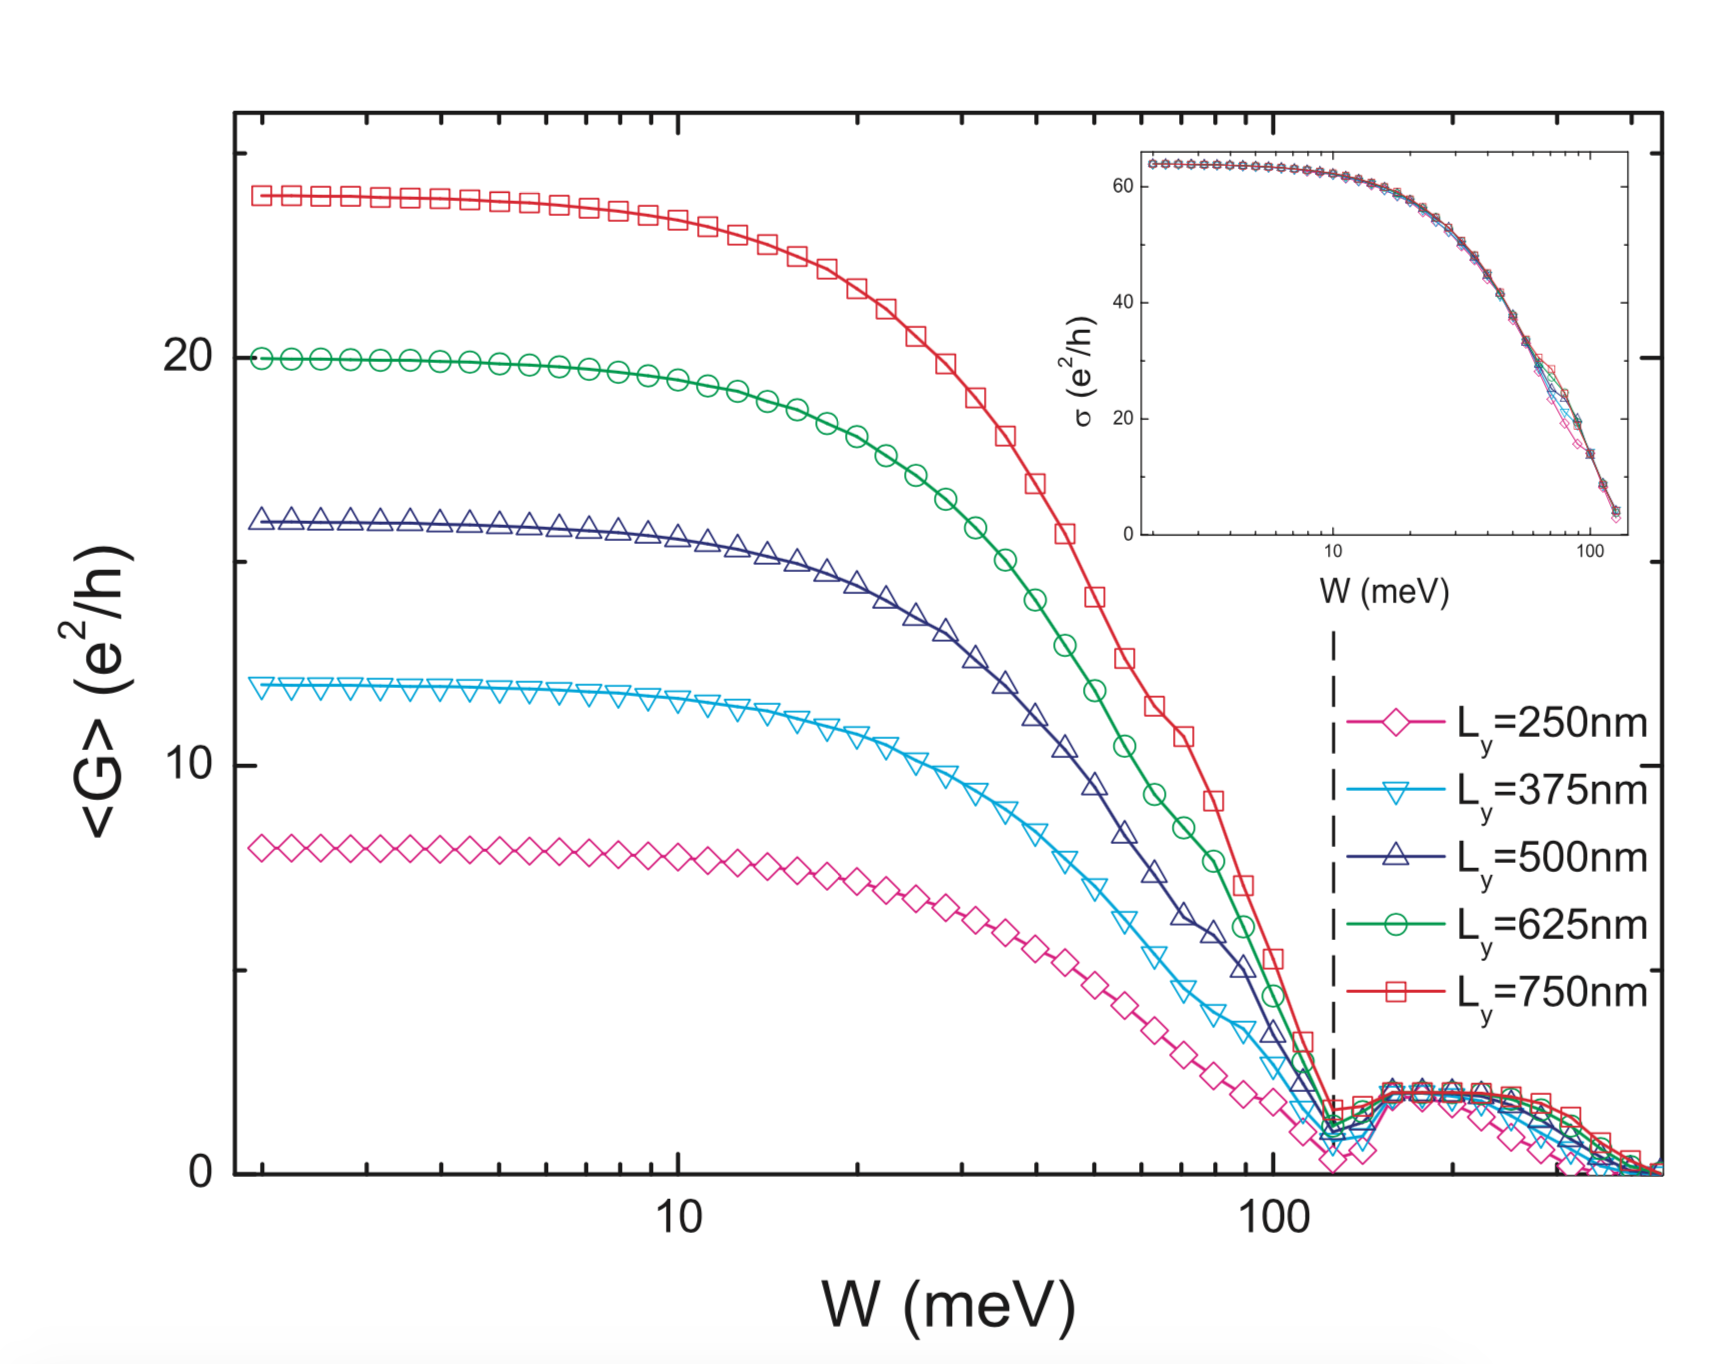
\includegraphics[width=\textwidth]{./media/expected-result.png}
\end{minipage}

\newpage
\section{Experimenting with disorder}
\begin{itemize}
  \item The physics of a topological insulator is unaffected by weak
  disorder, but is destroyed by large disorder
  \item BUT: Disorder can create a topological insulator for parameters where the system was metallic in 
  the absence of disorder
  \item These states are called topological Anderson insulators
  \item Disorder can be modeled as random on-site energy with a uniform distribution within $[-W_0, W_0]$
\end{itemize}

\newpage
\begin{equation*}
  t_{ij} \rightarrow t_{ij} \times \exp\left(i \frac{e}{\hbar} \int_{\mathbf{x}_j}^{\mathbf{x}_i} \mathbf{A}(\mathbf{x}) d\mathbf{s}\right)
  = \exp\left(i\, 2 \pi \frac{\phi}{\phi_0} \frac{(y_i + y_j)(x_i-x_j)}{2a^2} \right) \textrm{, where}~\phi = B a^2
\end{equation*}
\begin{equation*}
  V_\text{dis} = \sum_i W_i \ket i \bra i
\end{equation*}
\begin{equation*}
  \mathcal H = \sum\limits_i V_{\textrm{dis}}\ket i \bra i + \sum\limits_{<i,j>} t_{ij} \ket i \bra j
\end{equation*}

\begin{figure}[h!]
  \begin{center}
  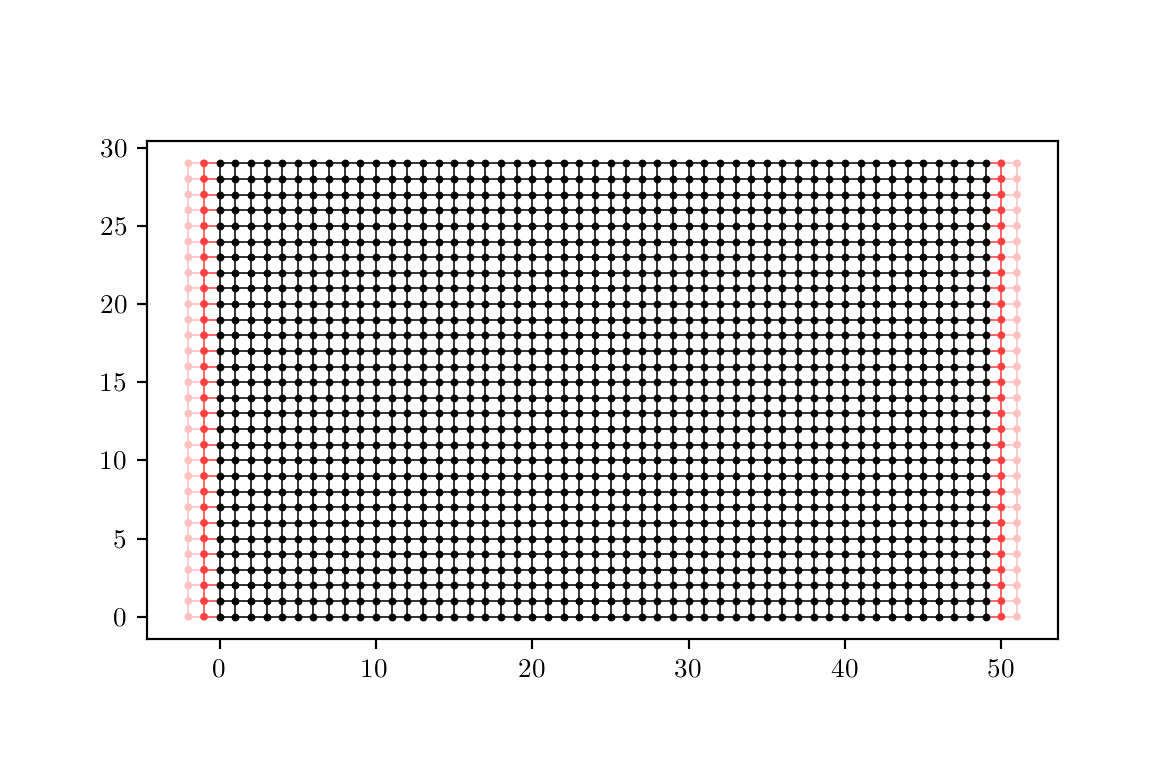
\includegraphics[height=0.55\textheight]{./media/square_lattice_W=30_L=50.png}
  \caption{Creating a simple square lattice}
  % \label{fig:peierls}
  \end{center}
\end{figure}

\newpage
\begin{figure}
  \centering
  \begin{minipage}{0.49\textwidth}
    \centering
    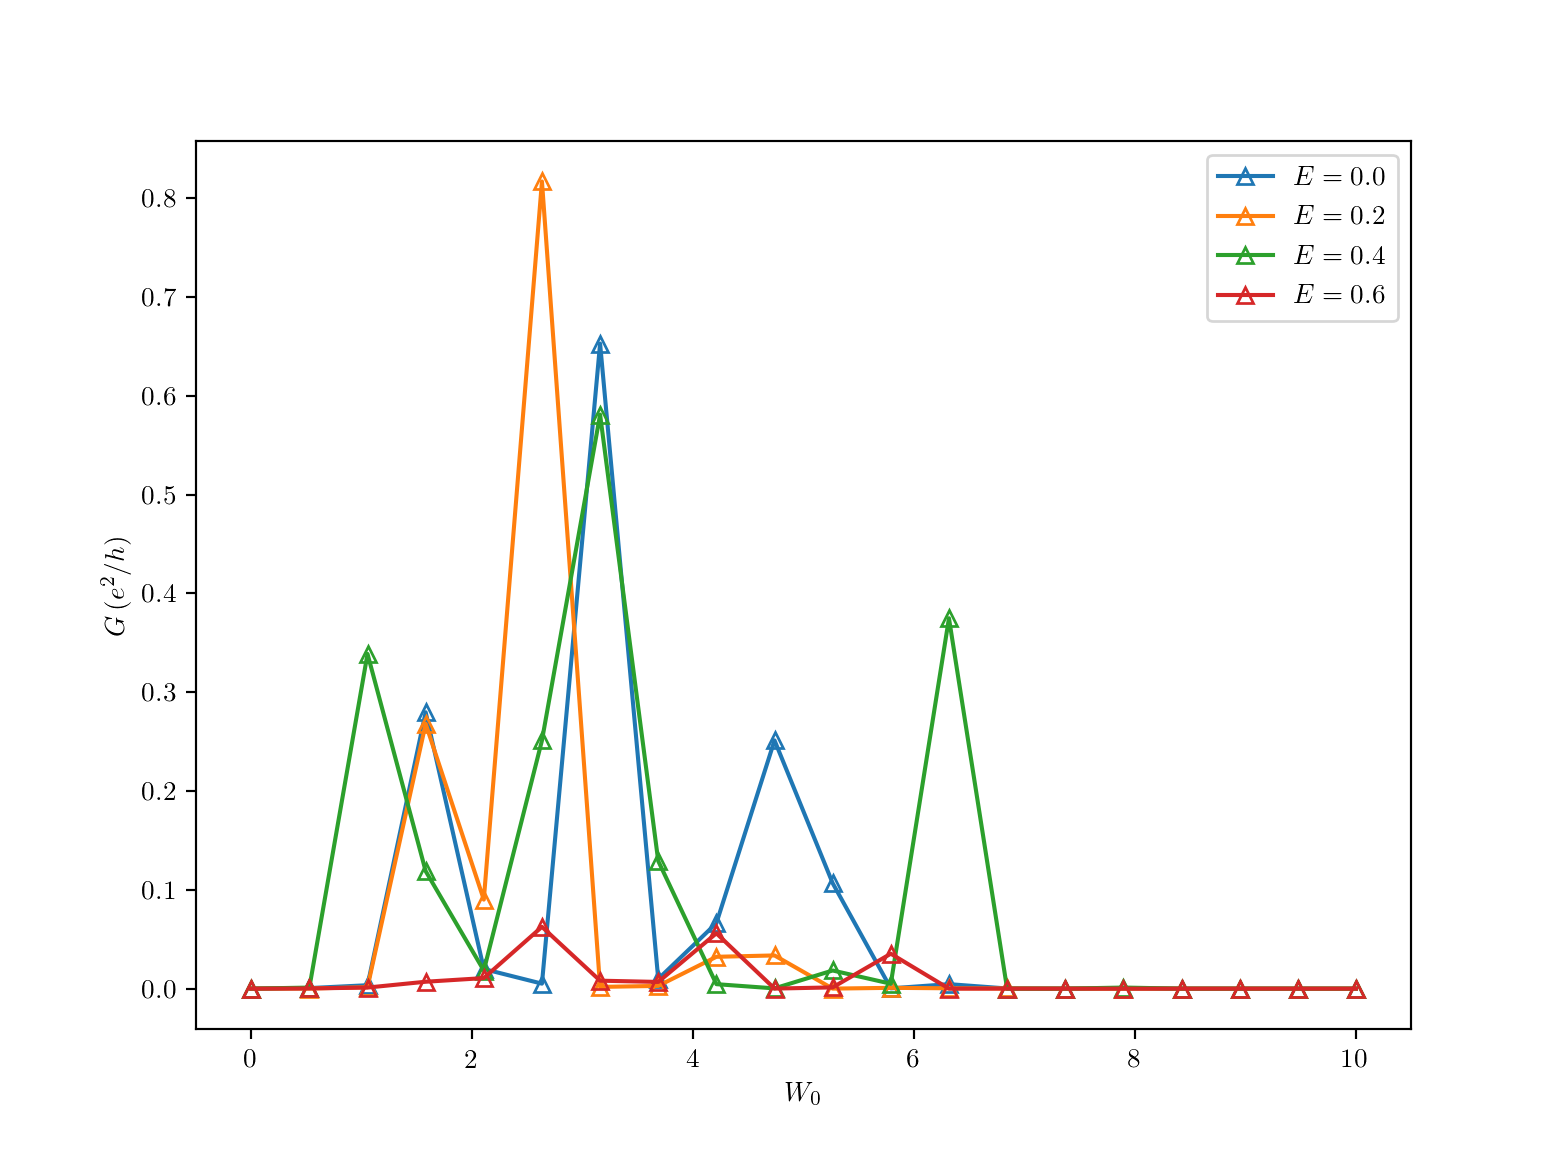
\includegraphics[width=1.0\textwidth]{./media/transmission_square_lat_phi=0dot0.png} % second figure itself
    \caption{Transmission in function of disorder for $\phi=0$}
  \end{minipage}\hfill
  \begin{minipage}{0.49\textwidth}
      \centering
      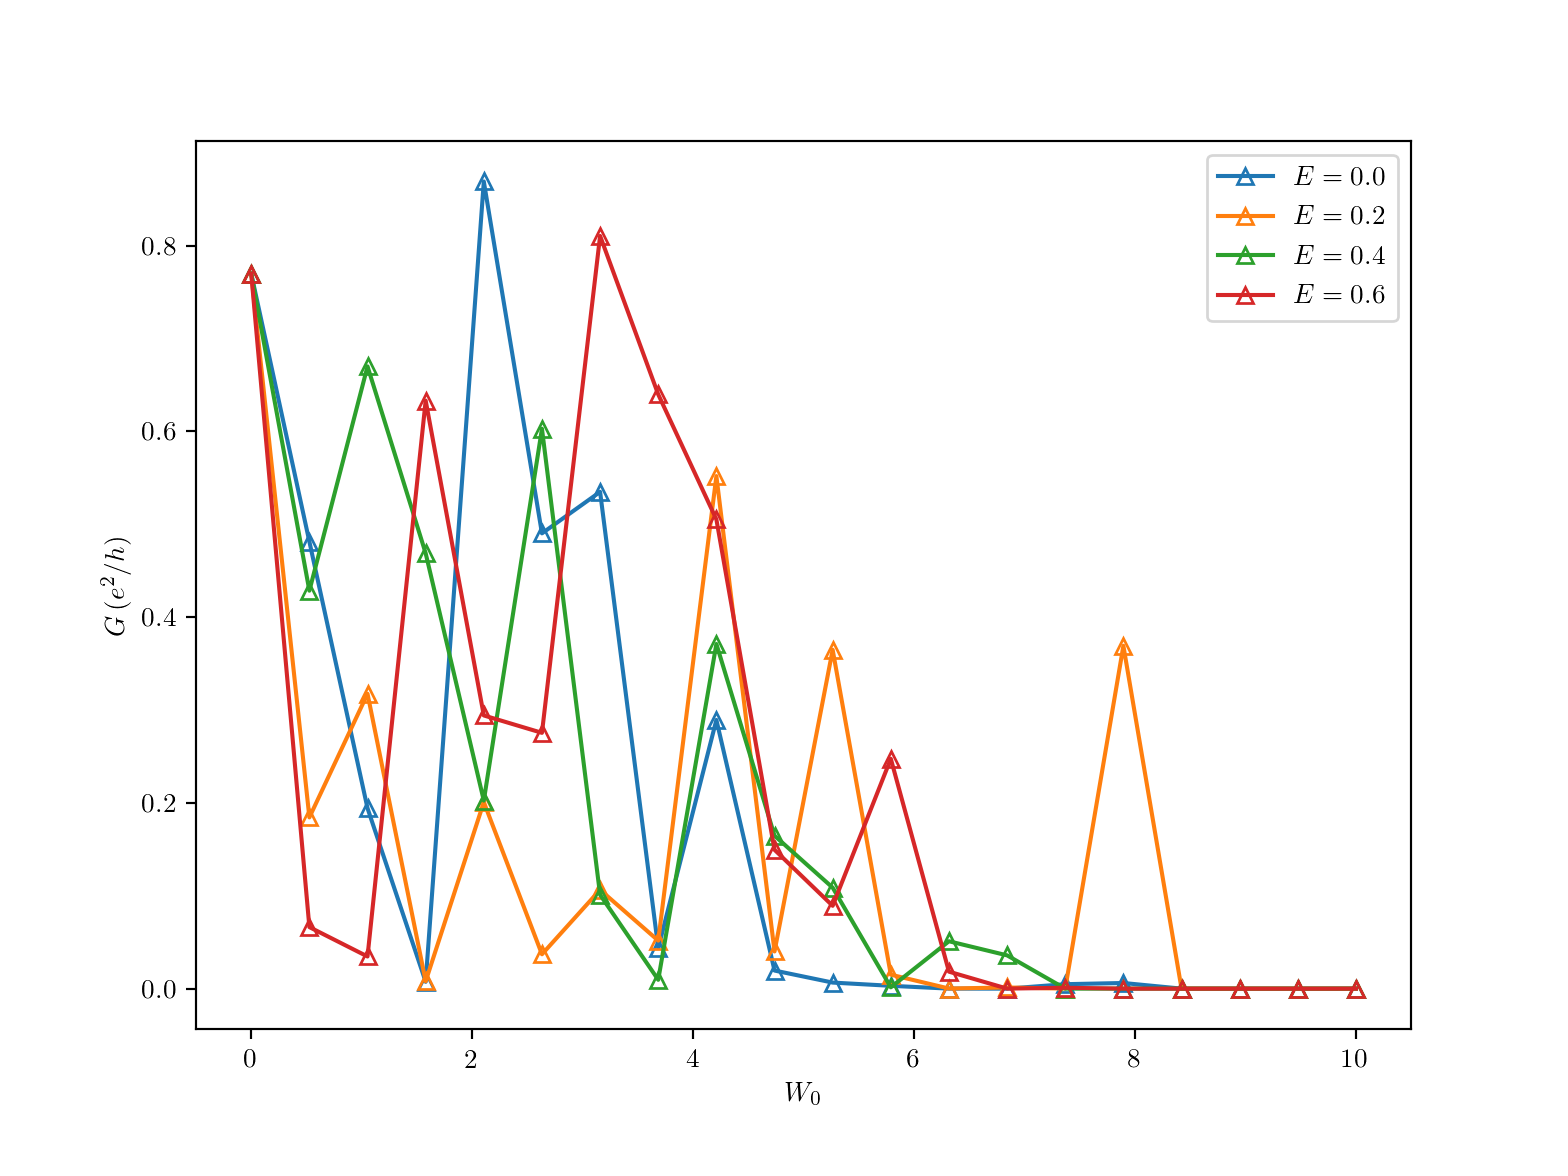
\includegraphics[width=1.0\textwidth]{./media/transmission_square_lat_phi=0dot2.png} % first figure itself
      \caption{Transmission in function of disorder for $\phi=0.2$}
  \end{minipage}
\end{figure}

\newpage
\begin{figure}[h!]
  \begin{center}
  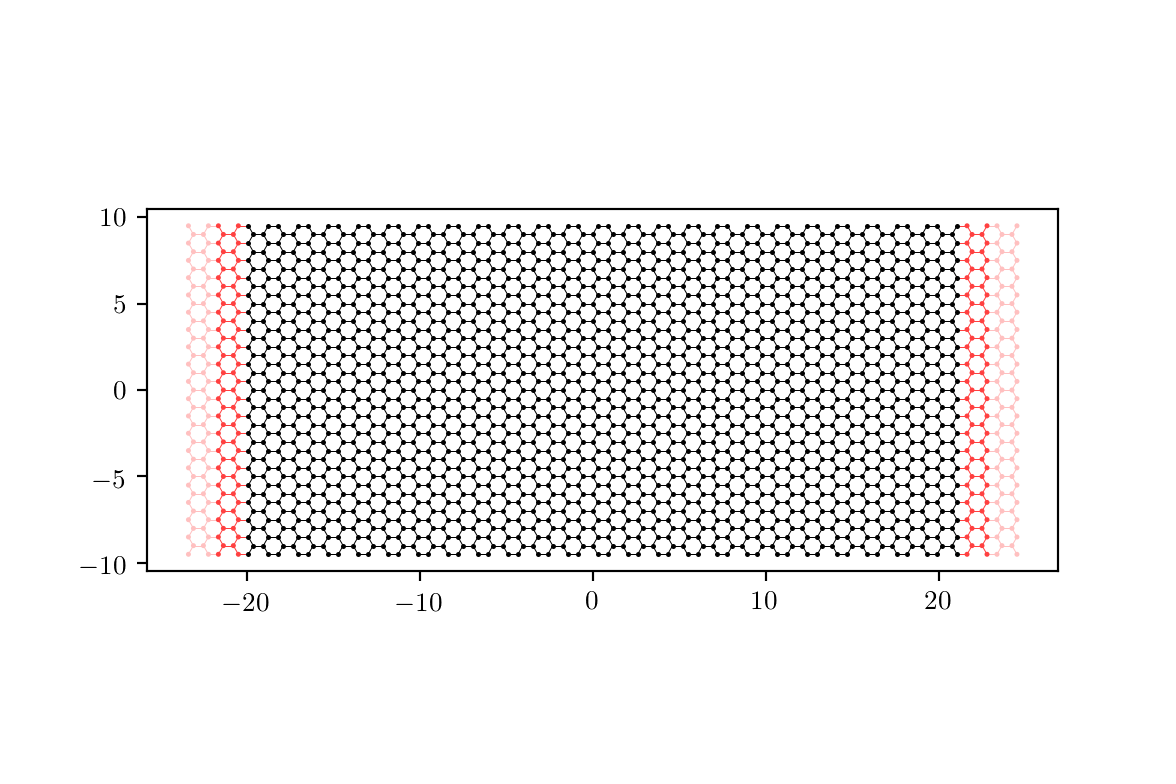
\includegraphics[height=0.85\textheight]{./media/graphene_lattice_W=20_L=40.png}
  \caption{Simple graphene lattice}
  % \label{fig:peierls}
  \end{center}
\end{figure}

\newpage
\begin{figure}[h!]
  \begin{center}
  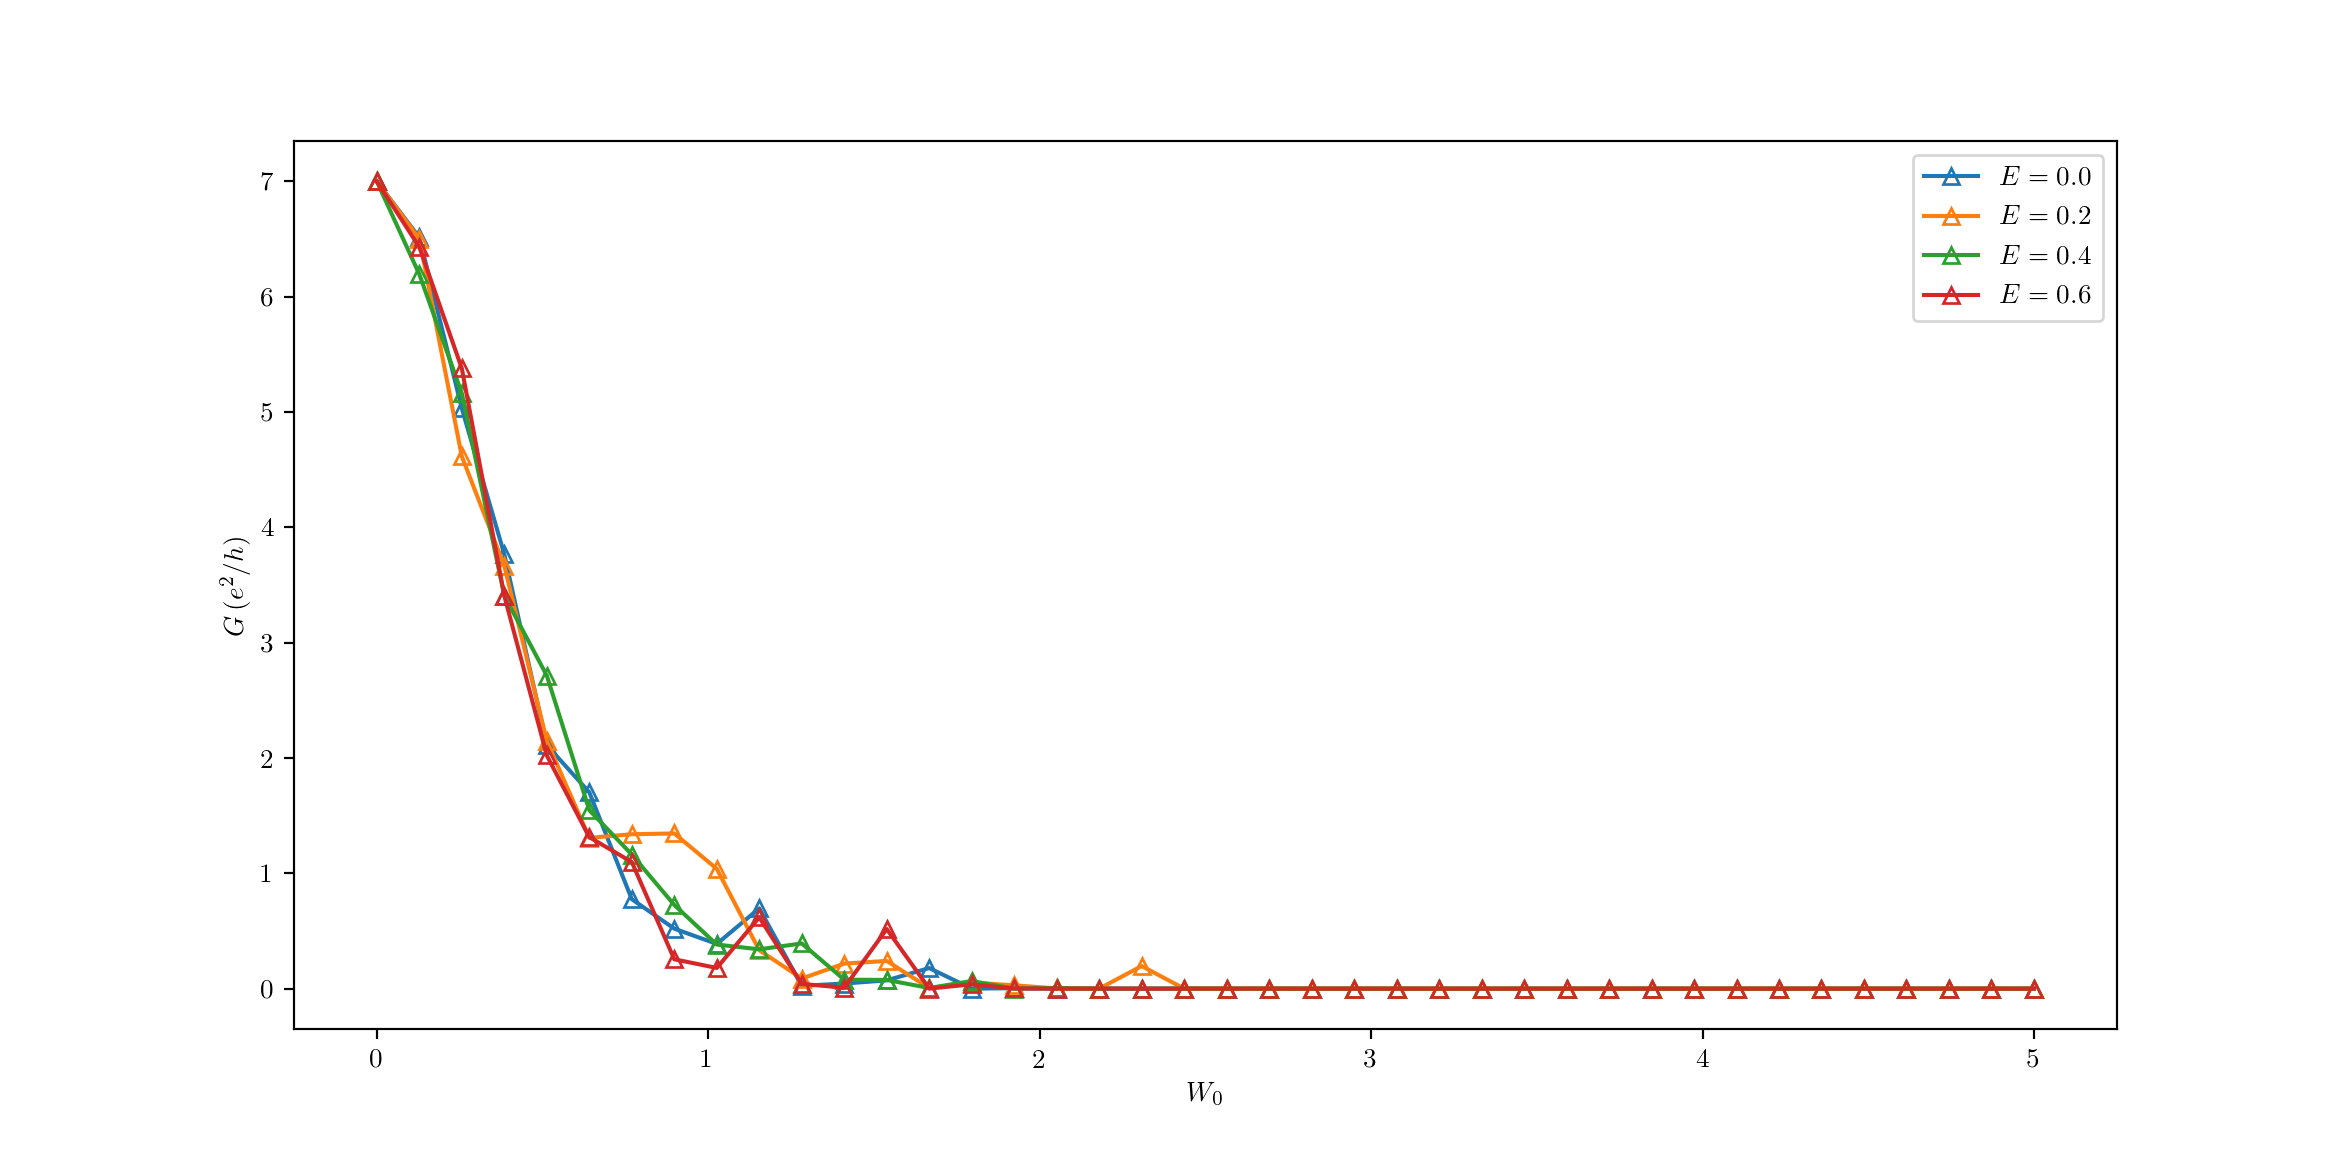
\includegraphics[height=0.85\textheight]{./media/transmission_graphene_lat_phi=0dot0Wmax=5.png}
  \caption{Transmission in function of disorder for $\phi=0$}
  % \label{fig:peierls}
  \end{center}
\end{figure}
\begin{figure}[h!]
  \begin{center}
  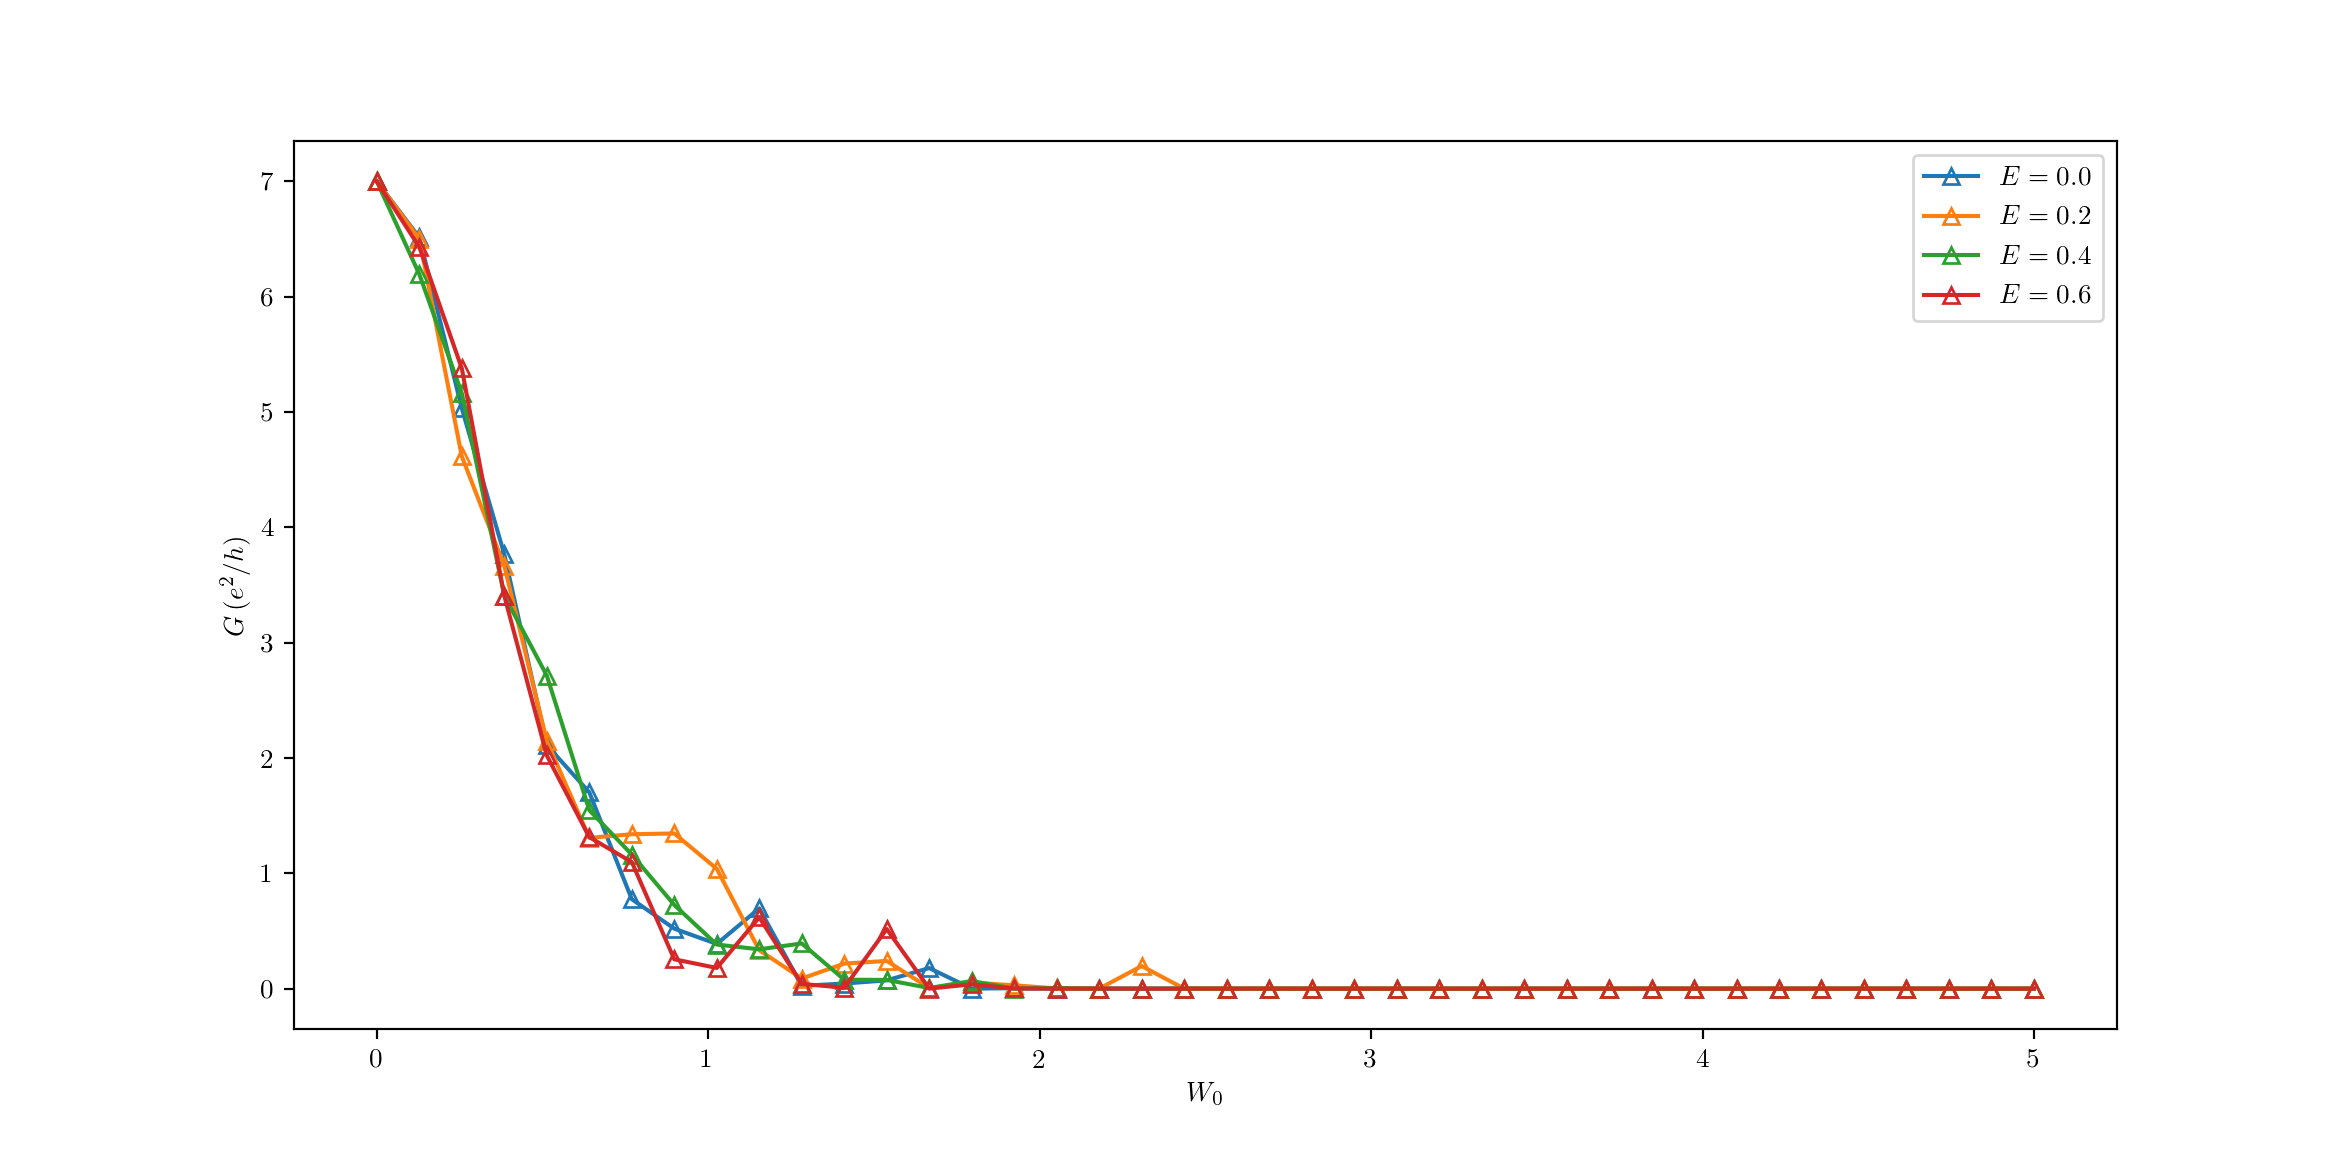
\includegraphics[height=0.85\textheight]{./media/transmission_graphene_lat_phi=0dot0Wmax=5.png}
  \caption{Transmission in function of disorder for $\phi=0.2$}
  % \label{fig:peierls}
  \end{center}
\end{figure}


\newpage
\begin{figure}[h!]
  \begin{center}
  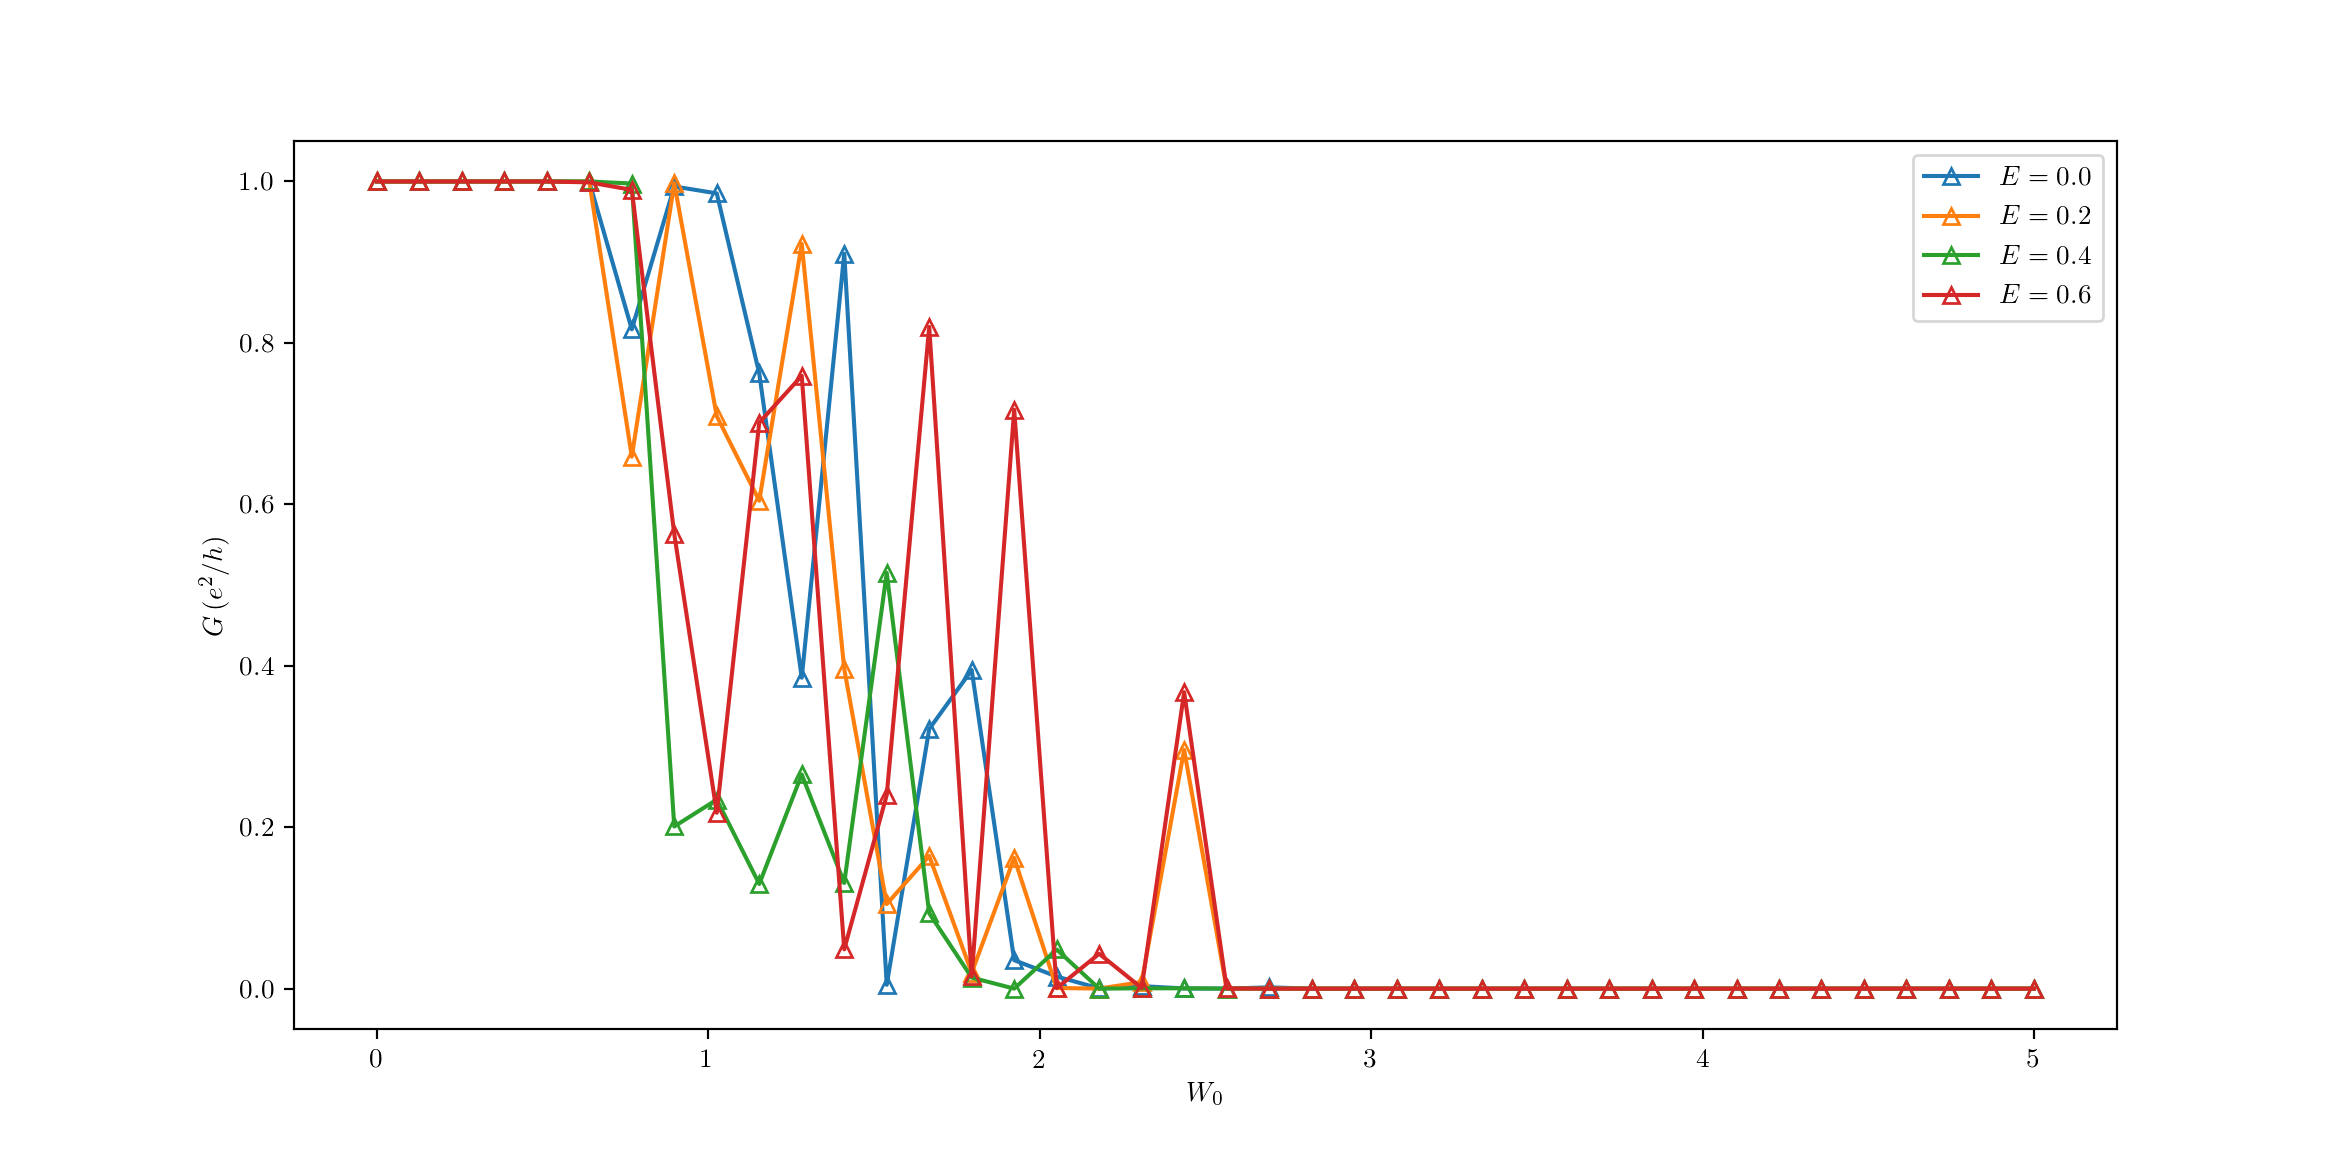
\includegraphics[height=0.85\textheight]{./media/transmission_graphene_lat_phi=0dot4Wmax=5.png}
  \caption{Transmission in function of disorder for $\phi=0.4$}
  % \label{fig:peierls}
  \end{center}
\end{figure}
\begin{figure}[h!]
  \begin{center}
  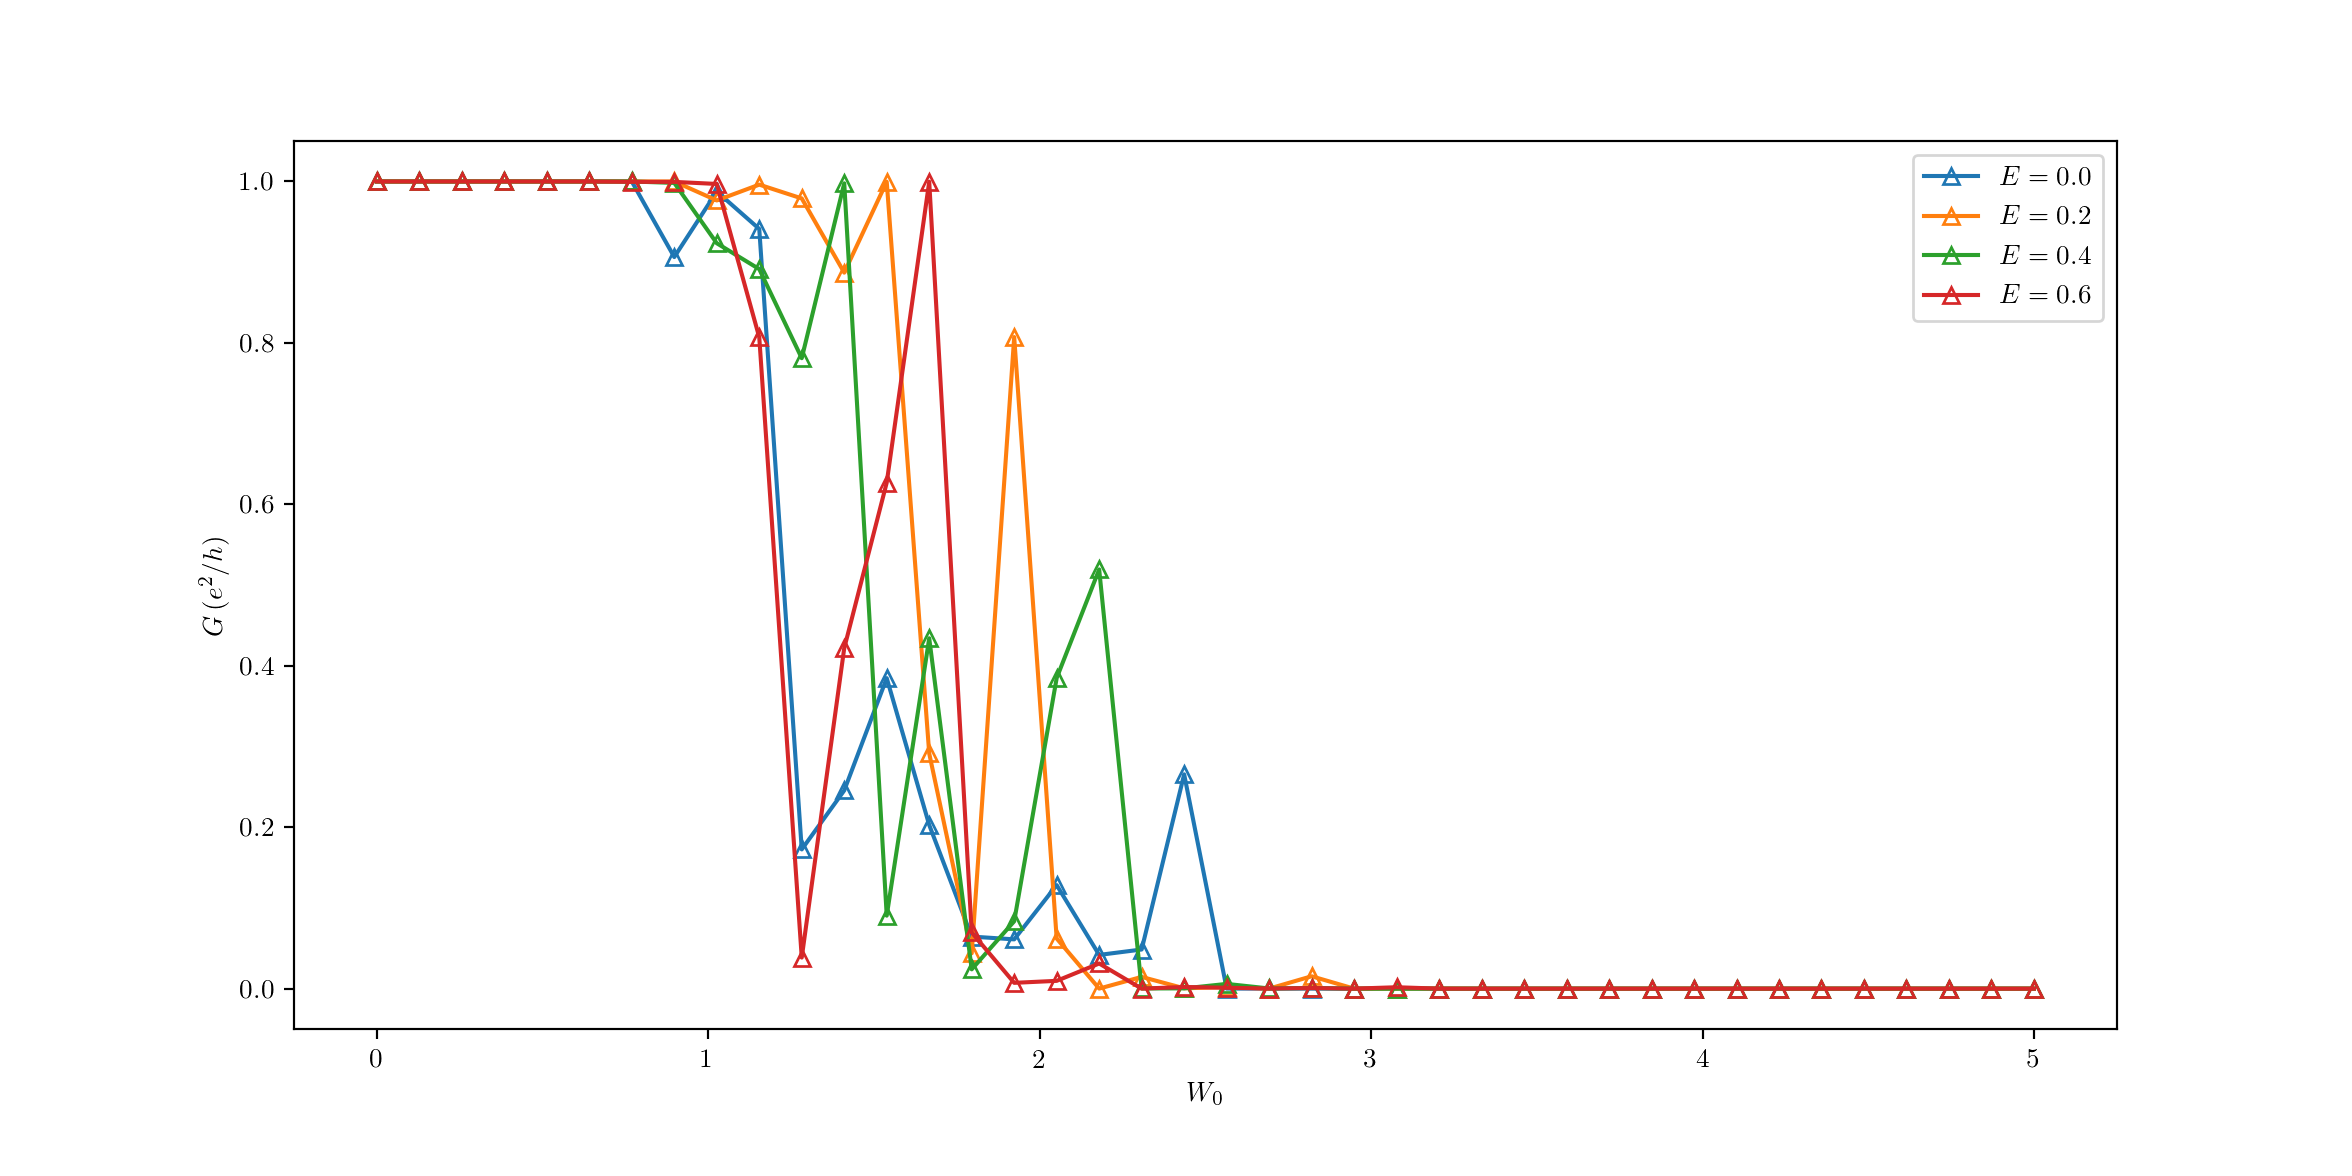
\includegraphics[height=0.85\textheight]{./media/transmission_graphene_lat_phi=0dot6Wmax=5.png}
  \caption{Transmission in function of disorder for $\phi=0.6$}
  % \label{fig:peierls}
  \end{center}
\end{figure}

\newpage
\section*{Next step}
The article about TAI (\url{https://arxiv.org/abs/0811.3045}) specifies the Hamiltonian for HgTe/CdTe:
\begin{equation*}
  \mathcal H(\bb k) = \left(
    \begin{array}{cc}
      h(\bb k) & 0 \\
      0 & h^{\dagger}(-\bb k) 
    \end{array}
    \right)
\end{equation*}
\begin{equation*}
  h(\bb k) = \epsilon(k) + \bb d (\bb k)\bb\sigma \textrm{, } \, \bb k = (k_x, k_y) 
\end{equation*}
\begin{equation*}
  \bb d(\bb k ) = (Ak_x, Ak_y, M-Bk^2) \textrm{; } \, \epsilon(k) = C-Dk^2
\end{equation*}
Problem:
\begin{itemize}
  \item Kwant builders accept only scalars or matrices that are in real space, not in $\bb k$-space.
  \item How can I implement the above Hamiltonian in kwant?
\end{itemize}

\begin{figure}[h!]
  \begin{center}
  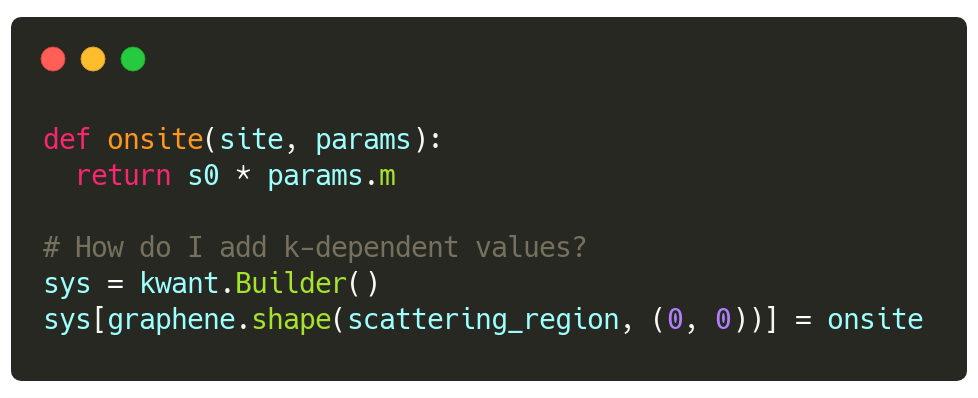
\includegraphics[width=0.85\textwidth]{./media/k-space-problem.png}
  % \caption{Transmission in function of disorder for $\phi=0.6$}
  % \label{fig:peierls}
  \end{center}
\end{figure}
\end{document}
